\newpage
\section{Hyperbole}

\subsection{Définition bifocale}\label{section:hypbifo}
De la même manière qu'avec l'ellipse, il est possible de faire le lien entre le cône coupé et la définition bifocale de l'hyperbole.

\begin{tcolorbox}[colback=cyan!5, colframe=cyan!70!blue, title=Définition bifocale de l'hyperbole]
\defn{Soient $F_1$ et $F_2$ deux points distincts d’un plan $\Pi$, distants de $\overline{F_1F_2} = 2c$. \\
Une hyperbole de foyers $F_1$ et $F_2$ est le lieu des points $M$ du plan $\Pi$ tels que la valeur absolue de la différence des distances de $M$ à $F_1$ et $F_2$ est constante, et strictement inféreure à la distance $\overline{F_1F_2}=2c $.}

\begin{equation}
    \mathcal{H}=\left\{\, M \in \Pi \;\middle|\; 
|\overline{MF_1} - \overline{MF_2}| = 2a \right\},
\end{equation}


où $a >0 $ est une constante vérifiant $2a < 2c.$
\end{tcolorbox}

\begin{figure}[H]
    \centering
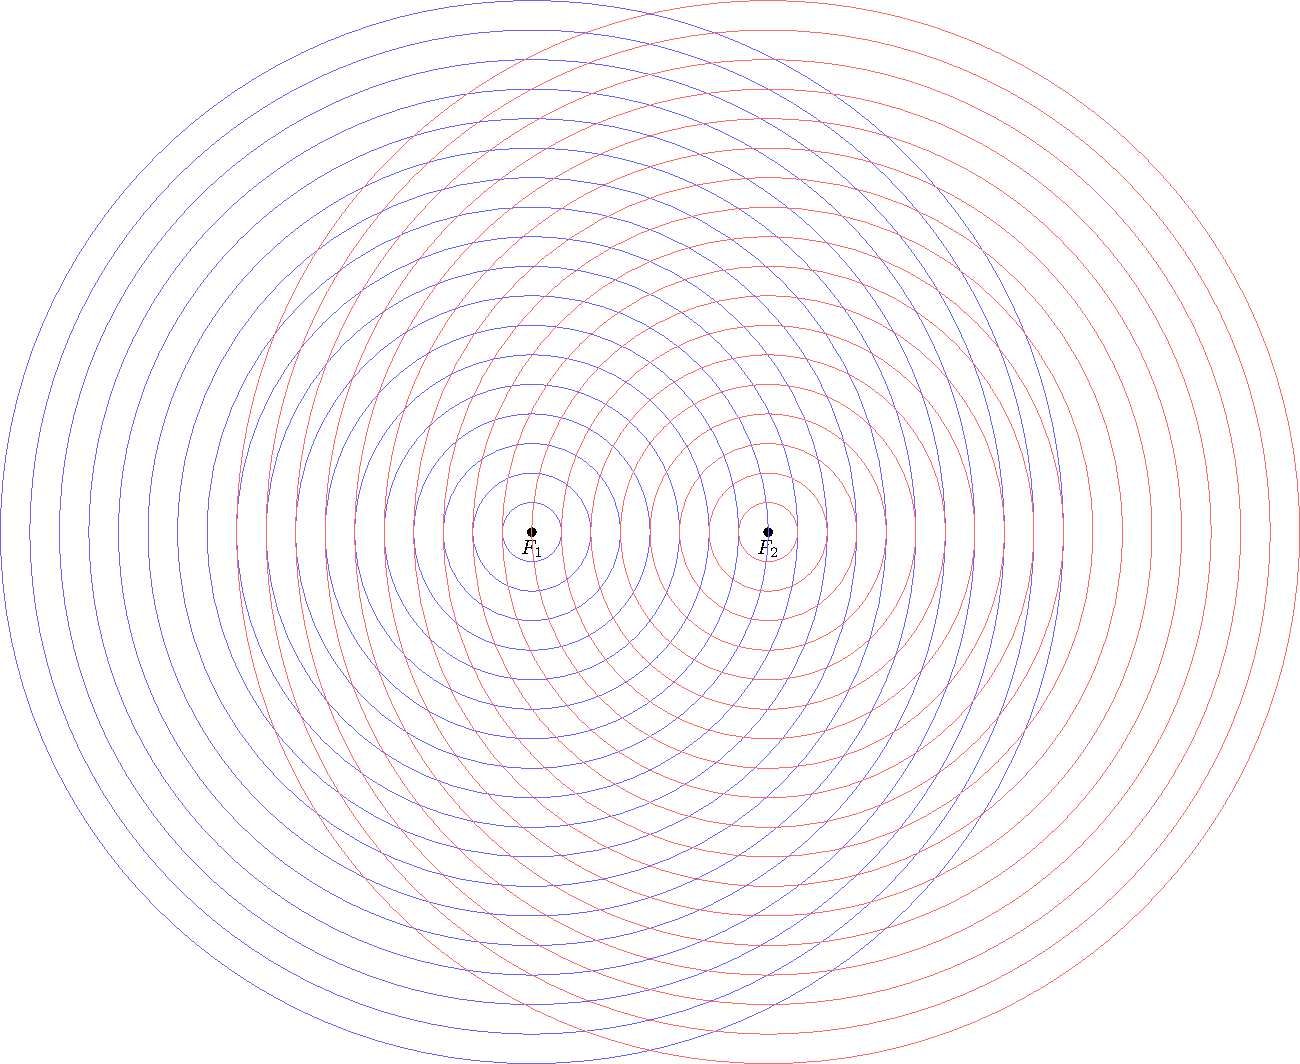
\includegraphics[scale = 0.73]{sections/tikz_standalone/hyp_1.pdf}
\end{figure}
\normalfont
A partir de cette définition, tracez une hyperbole avec $2a = 3$ unités de longueur.\\
Sans guide tracé, sauriez-vous le refaire avec un compas ?
\newpage

\begin{figure}[H]
\centering
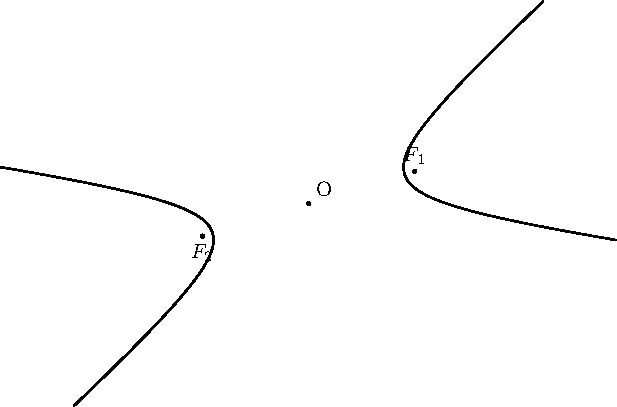
\includegraphics[scale = 0.8]{sections/tikz_standalone/hyp_2.pdf}

\end{figure}
\begin{tcolorbox}[colback=cyan!5, colframe=cyan!70!blue, title=Vocabulaire de l'hyperbole]

Le \textbf{centre} d'une hyperbole est le milieu du segment $[F_1F_2]$ reliant les deux foyers.\\
Un \textbf{diamètre} d'une hyperbole est toute droite passant par le centre de l'hyperbole.\\
L' \textbf{axe focal ou transverse} d'une hyperbole est la droite $F_1F_2$ passant par les deux foyers.\\ 
L' \textbf{axe non focal} d'une hyperbole est l'axe qui est la médiatrice de $[F_1F_2]$.\\ 
La \textbf{distance focale} d'une hyperbole est la distance $\overline{F_1F_2} = 2c$ entre les deux foyers.\\
Les \textbf{sommets} $S_1, S_2$ d'une l'hyperbole sont les points d'intersection de l'hyperbole avec son axe focal.\\

\end{tcolorbox}

\begin{tcolorbox}[colback=magenta!5, colframe=red!50!blue, title=Propriétés de l'hyperbole]
L'hyperbole possède 2 axes de symétries : son axe focal et son axe non focal.\\
L'hyperbole possède 1 centre de symétrie : son centre.

\end{tcolorbox}



\begin{minipage}{0.5\textwidth}
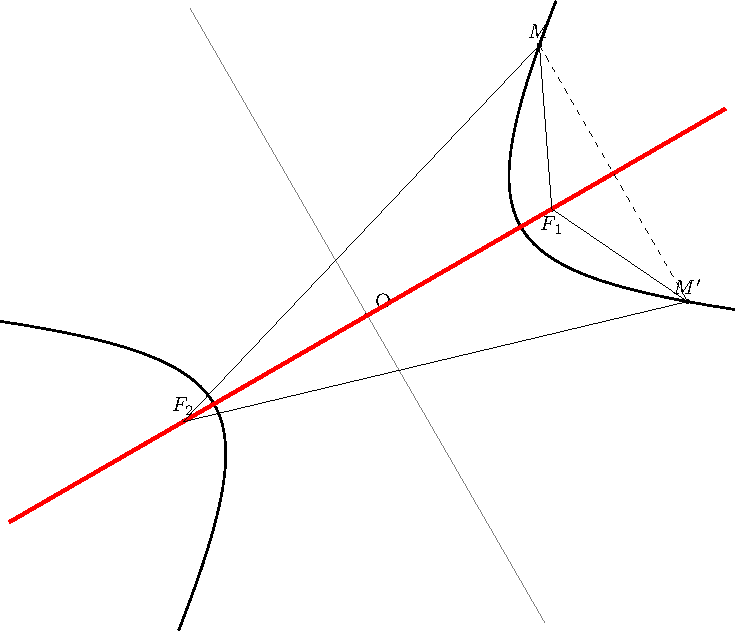
\includegraphics[scale = 0.5]{sections/tikz_standalone/hyp_4.pdf}
\end{minipage}
\hfill
\begin{minipage}{0.5\textwidth}
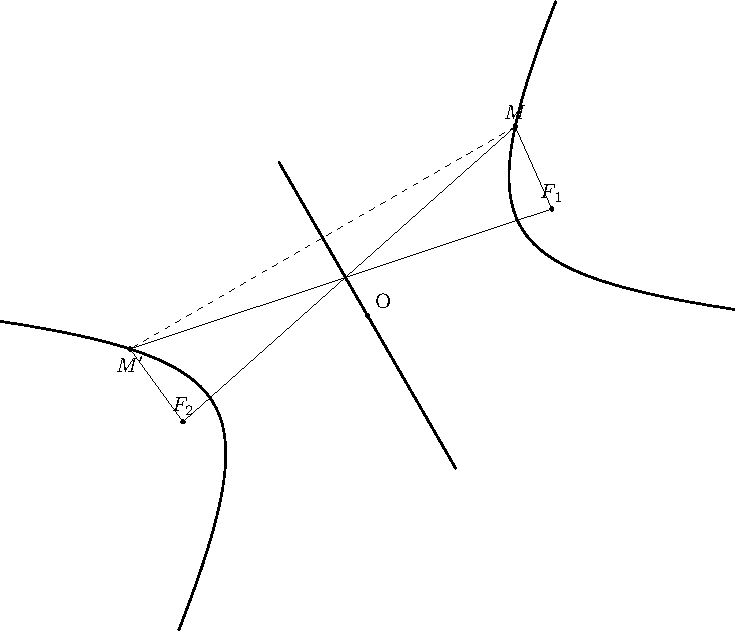
\includegraphics[scale = 0.5]{sections/tikz_standalone/hyp_3.pdf}
\end{minipage}

\vspace{1pt}
\hspace{0.3\textwidth}
\begin{minipage}{0.5\textwidth}
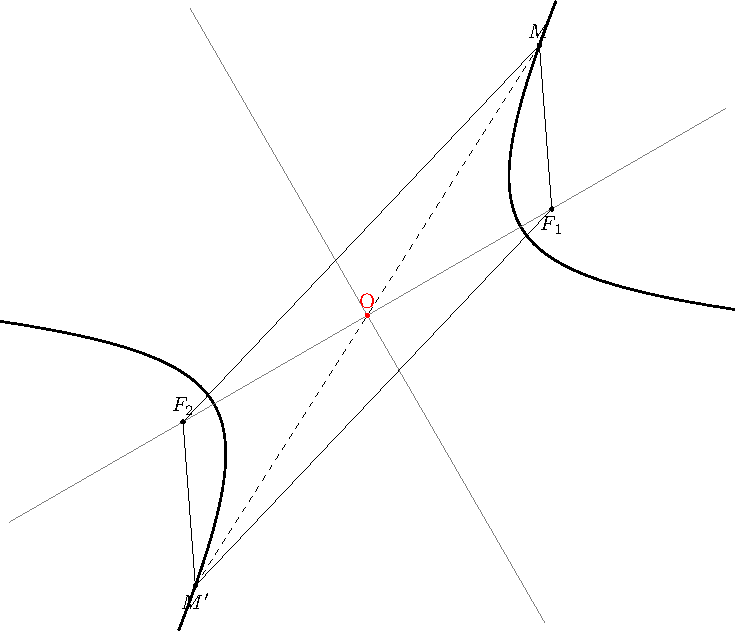
\includegraphics[scale = 0.45]{sections/tikz_standalone/hyp_5.pdf}

\end{minipage}
\hfill

\newpage
Choisissons à présent un repère orthonormé commode pour l'étude de l'hyperbole :\\
L'axe x est l'axe focal de l'hyperbole.\\
L'axe y est l'axe non focal de l'hyperbole.
\begin{figure}[H]
\centering

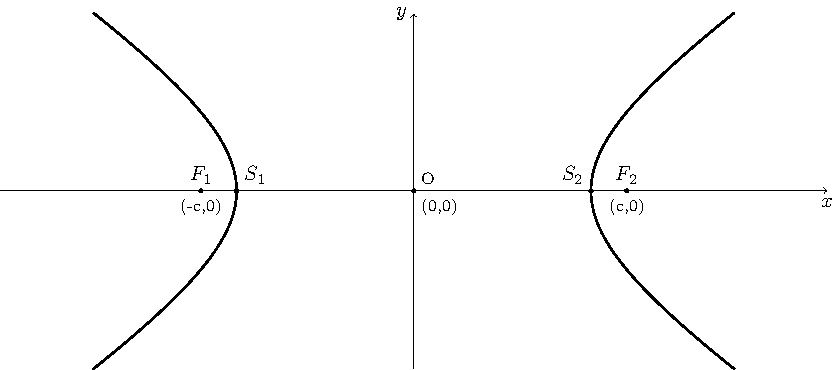
\includegraphics[scale = 1.1]{sections/tikz_standalone/hyp_6.pdf}
\end{figure}

\exo{Exprimez les coordonnées du sommet $S_2$ en fonction des longueurs connues. Déduisez ensuite les coordonnées de $S_1$.}

\begin{eleve}


\vspace{1cm}
\begin{minipage}{0.3\textwidth}
    \begin{align*}
&|\overline{S_2F_1} &-& \overline{S_2F_2}| &= 2a\\
&\overline{S_2F_1} &-& \overline{S_2F_2} &= 2a\\
&c+\overline{OS_2} &-&  (c-\overline{OS_2}) &= 2a\\
&&&\overline{OS_2} &= a
\end{align*}  
\end{minipage}
\vspace{1cm}

$S_2(a,0)$ et $S_1(-a,0)$

\end{eleve}

\newpage

Repartons à présent de la définition bifocale afin d'obtenir par la méthode de traduction une équation cartésienne dans ce repère choisi.


% Ellipse distance constante
\begin{figure}[H]
\centering
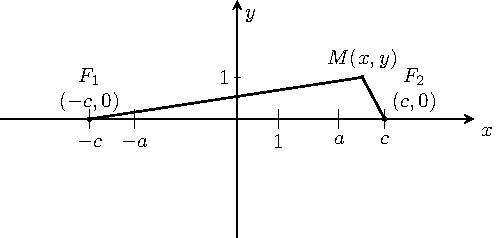
\includegraphics[scale = 1.3]{sections/tikz_standalone/hyp_7.pdf}
\end{figure}
\begin{tcolorbox}[colback=white, colframe=green!60!black,  boxrule=0pt, title=Démonstration de l'équation cartésienne de l'hyperbole à partir de sa définition bifocale.]
\end{tcolorbox}
\begin{eleve}
    
\begin{align*}
   && |\overline{MF_1} - \overline{MF_2}| &= 2a\\
    &\iff & \sqrt{(x+c)^2 + y^2} - \sqrt{(x-c)^2 + y^2} &= \pm 2a
\end{align*}\\
La différence des distances est positive lorsque le point $M$ est plus proche de $F_2$ que de $F_1$.
Le point $M$ fait alors partie de la branche droite de l'hyperbole.\\
La différence des distances est négative lorsque le point $M$ est plus proche de $F_1$ que de $F_2$.
Le point $M$ fait alors partie de la branche gauche de l'hyperbole.\\
\begin{align*}
    &\iff & \sqrt{(x+c)^2 + y^2} &= \pm 2a + \sqrt{(x-c)^2 + y^2}
\end{align*}


Pour éliminer les racines carrées, on peut élever les deux côtés au carré. 
Cependant, la fonction $x \mapsto  x^2$ n'est pas injective sur $\mathbb{R}$. 
Le fait de mettre au carré peut faire apparaître des solutions parasites.\\
Afin de conserver une équivalence, il faut analyser le signe des membres de l'équation. 
Le membre de gauche est positif. 
Il faudra alors s'assurer que le membre de droite l'est aussi.\\
On a alors 2 conditions :
\begin{align*}
\sqrt{(x+c)^2 + y^2} =  \pm 2a + \sqrt{(x-c)^2 + y^2} \notag\\
\iff
\begin{cases}
(\sqrt{(x+c)^2 + y^2})^2 &= (\pm 2a +\sqrt{(x-c)^2 + y^2})^2\\[2mm]
2a + \sqrt{(x-c)^2 + y^2} &\geq 0, \qquad x>0 \\[2mm]
-2a + \sqrt{(x-c)^2 + y^2} &\geq 0, \qquad x<0
\end{cases}
\end{align*}
La première condition est toujours satisfaite puisqu'on somme 2 distances.\\
La deuxième condition concerne le cas où $M$ est sur la 
branche gauche de l'hyperbole : \\
$\sqrt{(x-c)^2 + y^2}\geq 2a$. Il faudrait que la 
distance des points $M$ de la branche gauche au foyer $F_2$ soit supérieure ou égale à $2a$.
Le point $M$ , situé le plus proche de $F_2$, correspond au sommet $S_1(-a,0)$ calculé précédemment.
Ce sommet $S_1$ est situé à une distance $c+a$ du foyer $F_2$. Or $c>a$ donc $c+a > 2a$. 
Cette 2e condition est toujours vérifiée aussi.
\begin{align*}
    & & \sqrt{(x+c)^2 + y^2} &= \pm 2a + \sqrt{(x-c)^2 + y^2} \notag\\
&\iff&(x+c)^2 + y^2 &= 4a^2 \pm 4a\sqrt{(x-c)^2 + y^2}+ (x-c)^2 + y^2\\
&\iff& \pm a\sqrt{(x-c)^2 + y^2} &= cx - a^2
\end{align*}
On peut élever au carré pour éliminer la racine carrée. Il faudra à nouveau faire attention à l'équivalence 
des équations.
\begin{align*}
 \pm a\sqrt{(x-c)^2 + y^2} = cx - a^2 \notag\\
    \iff \begin{cases}
        (a\sqrt{(x-c)^2 + y^2})^2 = (cx - a^2)^2\\[2mm]
    cx - a^2\leq0, \qquad (x<0)\\[2mm]
    cx - a^2\geq0, \qquad (x>0)
    \end{cases}
\end{align*}

Pour la branche de gauche ($x<0$), le membre de gauche est négatif ($a>0$ et racine carrée). 
Il faudra alors que le terme de droite soit également négatif : $cx - a^2\leq0$.\\
Comme $x$ est négatif et $c$ positif, la condition est toujours vérifiée.\\
Pour la branche de droite ($x>0$), le membre de gauche est positif ($a>0$ et racine carrée). 
Il faudra alors que le terme de droite soit également positif : $x\geq \dfrac{a^2}{c}$.\\
Cette condition est également vérifiée car le point $M$ ayant l'abscisse minimale sur cette branche est le sommet $S_2(a,0)$.
Comme $c>a$, on a bien  $a\geq \dfrac{a^2}{c}$.

On élève alors au carré :
\begin{align*}
\pm a\sqrt{(x-c)^2 + y^2} &= cx - a^2 \notag\\
a^2(x-c)^2 + a^2y^2 &= c^2x^2 - 2a^2cx+ a^4\\
(c^2- a^2)x^2 - a^2y^2 &= a^2(c^2- a^2)
\end{align*}
Comme $c>a$, on peut poser $b^2 = c^2 - a^2$ avec $b>0$. On a alors :
\begin{equation*}
    \mathcal{H} \equiv b^2x^2 - a^2y^2 = a^2b^2
\end{equation*}
\end{eleve}
\begin{tcolorbox}[colback=cyan!5, colframe=cyan!70!blue, 
title=Équation cartésienne réduite de l'hyperbole (rapportée à ses axes)]
Soient $a, c \in \mathbb{R}^+_0$ tels que $c > a$.\\
Dans un repère orthonormé, considérons une hyperbole de foyers 
$F_1(-c,0)$ et $F_2(c,0)$, et dont la différence des distances à chaque foyer 
est constante et égale à $2a$.\\ Alors son équation cartésienne réduite s'écrit :
\begin{equation}
\mathcal{H} \equiv \dfrac{x^2}{a^2} - \dfrac{y^2}{b^2} = 1
\label{eq:HypRed}
\end{equation}
avec 
\[
b^2 = c^2 - a^2.
\]
\end{tcolorbox}


\vspace{0.5cm}

\begin{minipage}{0.7\textwidth}
    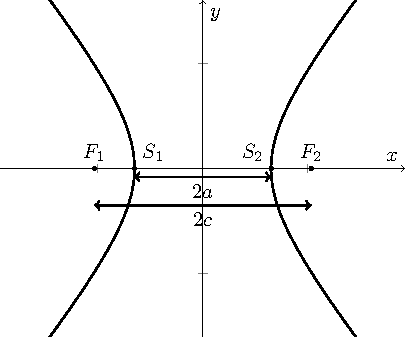
\includegraphics[scale = 1.2]{sections/tikz_standalone/hyp_8.pdf}

\end{minipage}
\hfill


\exth{$\dfrac{x^2}{16} - \dfrac{y^2}{9} = 1$}

\begin{minipage}{0.5\textwidth}
    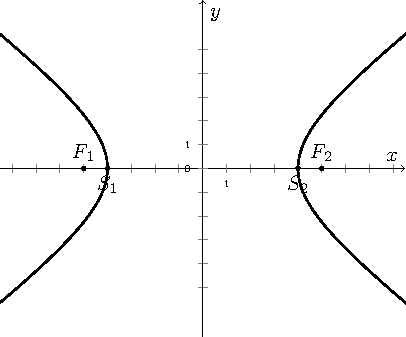
\includegraphics[scale = 1.2]{sections/tikz_standalone/hyp_9.pdf}
\end{minipage}
\hfill
\begin{minipage}{0.4\textwidth}
   \begin{eleve}
    Comme cet exemple d'hyperbole est rapportée à ses axes:\\
    Le centre est $(0,0)$\\
    L'axe focal est l'axe des abscisses\\
    L'axe non focal est l'axe des ordonnées\\


    La distance focale est 10 (unités de longueur)\\
    Les sommets sont $S_1(-4,0)$, $S_2(4,0)$\\
    \end{eleve}
\end{minipage}

\newpage

\subsection{Etude fonctionnelle et graphique}\label{section:hypgraphe}


L'équation de l'hyperbole (\ref{eq:EllRed}) n'est pas une équation de fonction.\\
Cependant, il est possible d’étudier sa représentation graphique en la décomposant en deux fonctions correspondant aux parties supérieure et inférieure de l’ellipse :\\
\[f_1 : \mathbb{R} \rightarrow\mathbb{R} : x \rightarrow \dfrac{b}{a}\sqrt{x^2-a^2} \]
\[f_2 : \mathbb{R} \rightarrow\mathbb{R} : x \rightarrow -\dfrac{b}{a}\sqrt{x^2-a^2} \]

\exo{Analysez la fonction $f_1$, sa dérivée première, sa dérivée seconde et son graphe.}
\begin{eleve}
\textbf{Etude de $f_1$}\\
Domaine : dom $f_1 = \leftarrow; -a]\cup  [a, \rightarrow$\\
\\~
Asymptotes ?

$G_{f_1}$ n'admet pas d'asymptote verticale car le domaine est un intervalle fermé.

$\lim_{x\rightarrow+\infty} f_1(x) = +\infty$

$G_{f_1}$ n'admet pas d'asymptote horizontale.

$\lim_{x\rightarrow+\infty} \dfrac{f_1(x)}{x} = \lim_{x\rightarrow+\infty} \dfrac{b}{a}\sqrt{1-\dfrac{a^2}{x^2}} = \dfrac{b}{a}$

$\lim_{x\rightarrow+\infty} f_1(x) - \dfrac{b}{a}x = 
\lim_{x\rightarrow+\infty} \dfrac{b}{a}(\sqrt{x^2-a^2} -x)\dfrac{\sqrt{x^2-a^2} +x}{\sqrt{x^2-a^2} +x} = \lim_{x\rightarrow+\infty} \dfrac{b}{a}\dfrac{(x^2-a^2 - x^2)}{\sqrt{x^2-a^2} +x} = 0$\\

Asymptote oblique à droite : $y = \dfrac{b}{a}x$

Asymptote oblique à gauche : $y = -\dfrac{b}{a}x$\\
\\~
Racines : $G_{f_1}\cap (Ox) = \{(-a,0), (a,0)\}$\\
Ordonnées à l'origine : $G_{f_1}\cap (Oy) = \{\emptyset\}$\\
\\~
Paire: $\forall x \in \text{dom}f_1, f(-x) = \dfrac{b}{a}\sqrt{(-x)^2 - (a)^2} = f(x)$.\\
On peut se limiter à l'étude de $f_1$ sur $[a,\rightarrow$.\\
\\~
Signe de $f_1$ sur $[a,\rightarrow$:

$
\begin{array}{c|c c c}
\hline
x & 0 & a &  \\
\hline
f(x) & \raisebox{-0.5\height}{\color{gray!50}\rule{1.5cm}{2cm}} &\makebox[1.5cm]{%
  %\color{white!100}\rule{0.5cm}{2cm}
  \raisebox{-0.5\height}{\color{gray!50}\rule{1.3cm}{2cm}}% grey area starts at center
  0
\raisebox{-0.5\height}{\color{white!50}\rule{0.55cm}{2cm}}
}  & +
   \\
\hline
\end{array}
$\\
\\~
\\~
\textbf{Etude de la dérivée première $f'_1$}\\
$f'_1(x) = \dfrac{bx}{a\sqrt{ x^2 - a^2}}$\\
Racines de $f'_1$ : $G_{f'_1}\cap (Ox) = \{\emptyset\}$\\
$\lim_{x\rightarrow a^+} f_1(x) = + \infty$.\\
Signe de $f'_1$ sur $[0,a]$:

$
\begin{array}{c|c c c}
\hline
x & 0 &  a &\\
\hline
f'(x) & \raisebox{-0.5\height}{\color{gray!50}\rule{1.3cm}{2cm}} &\makebox[1.5cm]{%
  %\color{white!100}\rule{0.5cm}{2cm}
  \raisebox{-0.5\height}{\color{gray!50}\rule{1.4cm}{2cm}}% grey area starts at center
  \raisebox{-0.5\height}{\rule{3pt}{2cm}}% vertical line
\raisebox{-0.5\height}{\color{white!50}\rule{0.55cm}{2cm}}
}  & +
   \\
\hline
\end{array}
$\\
\\~
\\~
\textbf{Etude de la dérivée seconde $f''_1$}\\
$f''_1(x) = \dfrac{-ab}{\sqrt{(x^2 - a^2)^3}}$\\
Racines de $f''_1$ : $G_{f''_1}\cap (Ox) = \{\emptyset\}$\\
Signe de $f''_1$ sur $[0,a]$:

$
\begin{array}{c|c c c}
\hline
x & 0 &  a &\\
\hline
f''(x) & \raisebox{-0.5\height}{\color{gray!50}\rule{1.3cm}{2cm}} &\makebox[1.5cm]{%
  %\color{white!100}\rule{0.5cm}{2cm}
  \raisebox{-0.5\height}{\color{gray!50}\rule{1.4cm}{2cm}}% grey area starts at center
  \raisebox{-0.5\height}{\rule{3pt}{2cm}}% vertical line
\raisebox{-0.5\height}{\color{white!50}\rule{0.55cm}{2cm}}
}  & -
   \\
\hline
\end{array}
$\\
\\~
\\~
\textbf{Tableau récapitulatif}\\
$
\begin{array}{c|c c c}
\hline
x & 0 &  a &\\
\hline
f'(x) & \raisebox{-0.5\height}{\color{gray!50}\rule{1.5cm}{2cm}} &\makebox[1.5cm]{%
  %\color{white!100}\rule{0.5cm}{2cm}
  \raisebox{-0.5\height}{\color{gray!50}\rule{1.5cm}{2cm}}% grey area starts at center
  \raisebox{-0.5\height}{\rule{3pt}{2cm}}% vertical line
\raisebox{-0.5\height}{\color{white!50}\rule{0.55cm}{2cm}}
}  & +
   \\
\hline
f''(x) & \raisebox{-0.5\height}{\color{gray!50}\rule{1.5cm}{2cm}} &\makebox[1.5cm]{%
  %\color{white!100}\rule{0.5cm}{2cm}
  \raisebox{-0.5\height}{\color{gray!50}\rule{1.5cm}{2cm}}% grey area starts at center
  \raisebox{-0.5\height}{\rule{3pt}{2cm}}% vertical line
\raisebox{-0.5\height}{\color{white!50}\rule{0.55cm}{2cm}}
}  & - \\
\hline
f(x) & \raisebox{-0.5\height}{\color{gray!50}\rule{1.5cm}{2cm}} &\makebox[1.5cm]{%
  %\color{white!100}\rule{0.5cm}{2cm}
  \raisebox{-0.5\height}{\color{gray!50}\rule{1.5cm}{2cm}}% grey area starts at center
  0
\raisebox{-0.5\height}{\color{white!50}\rule{0.55cm}{2cm}}
}  & \nearrow
   \\
 & & &\frown\\
\hline
\end{array}
$\\
\\~

\end{eleve}

\begin{figure}[H]
    \centering
    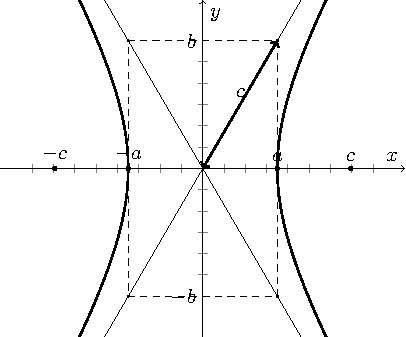
\includegraphics[scale = 0.8]{./sections/tikz_standalone/hyp_10.pdf}
\end{figure}

\newpage
\subsection{Définition monofocale}\label{section:hypmonofo}
